\documentclass[11pt,a4paper]{letter}
\usepackage[top=0.50in, bottom=0.5in, left=1.1in, right=1.1in]{geometry}
\usepackage{graphicx}

%\signature{}

\usepackage{Sweave}
\begin{document}

\begin{letter}{}

\includegraphics[width=0.3\textwidth]{logo_uah.png}

\opening{Dear Dr. Armarego-Marriot:} % EMW14Oct  -- I think you can address to the editor you've been corresponding with (but not critical). %IMC15OCT done

\noindent Please consider our paper, entitled `Phylogenetic estimates of species-level phenology improve ecological forecasting' as a Letter in \emph{Nature Climate Change}. Our research addresses the critical challenge of accurately predicting the impacts of climate change on plant phenology---with consequences for key ecosystem services---and highlights the importance of incorporating both species variability and phylogenetic information in forecasts.
\vspace{1.5ex}\\
Comments from three reviewers have greatly improved this manuscript and led us to present a suite of new analyses, which all reinforce our findings that including phylogenetic relationships improves ecological forecasting. Specifically, we have developed a new leave-one-clade-out cross-validation approach for hierarchical models (phylogenetic or non-phylogenetic) that confirms our finding that our phylogenetic model out-performs traditional hierarchical approaches. We also re-analysed our data with a new metric of chilling, and show our results are robust. In addition, we provide a more thorough description of our data and methods and discuss in more depth the implications of our research. 
\vspace{1.5ex}\\ % EMW14Oct -- careful: we have tree and shrub species, so talk about woody species .. I am also not sure they are ALL deciduous, which I think you may say some places (not a big deal, but we should check -- can you ask Dan B. to review? We don't need to wait for this I think, but should be *limited* in what we say... I wondered if some oak were evergreem). 
Our results are based on an unprecedented dataset on phenological responses to environmental cues (chilling, forcing and photoperiod) determined experimentally, which we collected systematically using standardized meta-analytic approaches. Reviewer 1 suggested increasing the geographic coverage of our dataset to southern hemisphere species, but there is extremely limited data available for this request (our methods had identified three studies, but they were rarely for non-domesticated species and could not be matched to high quality daily climate data, which we need for our approach). The papers suggested by Reviewer 1 report observational---not experimental---data and thus we cannot include them, unfortunately. We were aware of these limitations, which partly motivated us to develop the phylogenetic model we present here. Our results do include some Mediterranean species, but until further experiments on many more extra-temperate species are conducted, robust inferences well beyond the temperate zone will be difficult. We now discuss this briefly in the main text, as it is an important gap in the literature. % EMW14Oct  -- not sure what you meant here: until further experiments on extra-temperate species are conducted, quantifying uncertainty with Bayesian methods, and leveraging information on evolutionary relationships (which covary with biogeography) arise as an promising venue to generate robust predictions, even when departing from unbalanced data
\vspace{1.5ex}\\
We have addressed all reviewer concerns through substantial edits, corrections to the main text, and the addition of 5 new figures and 3 tables to the Supporting Information. We feel the new submission is much improved and detail our changes in the response letter to reviewers (note that reviewer comments are in \emph{italics}, while our responses are in regular text).  This manuscript is not under consideration elsewhere.  We hope that you will find it suitable for publication in \emph{Nature Climate Change}, and look forward to hearing from you.


\vspace{0.25ex}\\
\vspace{1.5ex}\\


\vspace{1.5ex}\\
\noindent Sincerely,\\
\vspace{1.5ex}\\
 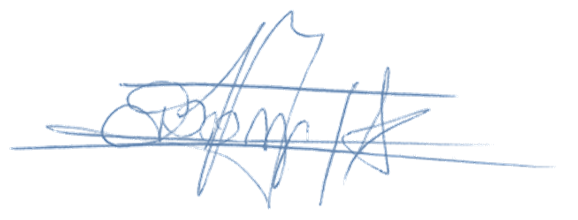
\includegraphics[width=0.2\textwidth]{Signature_IMC.png} \\
 \vspace{1.5ex}\\
\noindent Ignacio Morales-Castilla


\end{letter}
\end{document}
